%% The first command in your LaTeX source must be the \documentclass command.
\documentclass[acmtog]{acmart}
\usepackage[english,ngerman]{babel}
\usepackage[utf8]{inputenc} 

%% \BibTeX command to typeset BibTeX logo in the docs
\AtBeginDocument{%
  \providecommand\BibTeX{{%
    \normalfont B\kern-0.5em{\scshape i\kern-0.25em b}\kern-0.8em\TeX}}}
    
\copyrightyear{2024}
\acmYear{2024}
\citestyle{acmauthoryear}

\usepackage[figurename=Fig.]{caption}
\setcopyright{none}
\makeatletter
\renewcommand{\fnum@figure}{Abb. \thefigure}
\makeatother
\addto\captionsngerman{\renewcommand{\figurename}{Abb.}}
\settopmatter{printacmref=false} % Removes citation information below abstract
\renewcommand\footnotetextcopyrightpermission[1]{} % removes footnote with conference information in first column

%%
%% end of the preamble, start of the body of the document source.
\begin{document}

%%
%% The "title" command has an optional parameter,
%% allowing the author to define a "short title" to be used in page headers.
\title{Sicherheitsaspekte in der (agilen) Softwareentwicklung}

%%
%% The "author" command and its associated commands are used to define
%% the authors and their affiliations.
%% Of note is the shared affiliation of the first two authors, and the
%% "authornote" and "authornotemark" commands
%% used to denote shared contribution to the research.
\author{Finn Hoedt}
\authornote{Alle Studierenden trugen zu gleichen Teilen zu dieser Arbeit bei.}
\author{Maurice Raymond Putzger}
\authornotemark[1]
\author{Bastian Wecke}
\authornotemark[1]
\affiliation{%
  \institution{Hochschule für Technik, Wirtschaft und Kultur Leipzig (HTWK Leipzig)}
  \streetaddress{Karl-Liebknecht-Str. 132}
  \city{Leipzig}
  %\state{Ohio}
  \country{Deutschland}
  \postcode{04277}
}
%%
%% By default, the full list of authors will be used in the page
%% headers. Often, this list is too long, and will overlap
%% other information printed in the page headers. This command allows
%% the author to define a more concise list
%% of authors' names for this purpose.
\renewcommand{\shortauthors}{Hoedt, Putzger und Wecke}

%%
%% The abstract is a short summary of the work to be presented in the
%% article.
\begin{abstract}
  (Abstract-Länge ist typischerweise 15-25 Zeilen lang, in der PDF-Darstellung) 
  
  
\end{abstract}

\maketitle

\section{Einleitung und Motivation}

(Beschreibung von Kontext, Problemen, Anforderungen und Zielen) 



(kurze Zusammenfassung der Struktur der Belegarbeit)

Diese Arbeit ist folgendermaßen strukturiert. 
In Kapitel ... 
...
...
Abschließend ...

\section{Grundlagen}

Im Folgenden werden Begriffe zu den Themen Sicherheit und Shift-Left in der Softwareentwicklung erklärt, um somit eine grundlegende Wissensbasis für die danach folgenden Kapitel zu schaffen.

Als \textit{sichere Software} definieren wir solche, die den grundlegenden Prinzipien der Informationssicherheit \cite{blakley_information_2001} entspricht und auch trotz verschiedener Widrigkeiten in ihrer Funktionalität zuverlässig bleibt \cite{oueslati_literature_2015}. Diese Prinzipien werden in folgende Kategorien unterteilt:
\begin{enumerate}
    \item \textbf{Vertraulichkeit} beschreibt den Schutz sensibler Daten vor unbefugtem Zugriff.
    \item \textbf{Integrität} stellt sicher, dass die Daten konsistent und unverändert bleiben, außer sie werden bewusst durch autorisierte Nutzer verändert.
    \item \textbf{Verfügbarkeit} garantiert, dass die Software und ihre genutzten Daten und Ressourcen stets zugänglich sind. Die Verfügbarkeit muss auch unter gezielten Angriffen gewährleistet werden.
    \item \textbf{Zuverlässigkeit} ist ein System dann, wenn es sich zu jedem Zeitpunkt erwartungsgemäß verhält. Dies gilt ebenfalls unter etwaigen Widrigkeiten, wie beispielsweise unbefugten Zugriffen von außen.
\end{enumerate}
Diese vier Prinzipien bilden die Grundlage für sichere Software und müssen somit bei der Entwicklung von sicherheitskritischen Prozessen gezielt beachtet werden.\

Der \textit{Shift-Left} Ansatz beschreibt das Verschieben von Prozeduren bzw. Aktivitäten aus späteren Phasen des Software Development Life Cycle in Frühere \cite{andriadi_impact_2023}. An einer zeitlichen Achse, wie sie in der Abbildung \ref{fig:shiftleft} zu sehen ist, kann man die Verschiebung nach Links erkennen. Die Abbildung zeigt, wie der Fokus von der Softwarequalität von einem späteren Zeitpunkt in einen Früheren verlagert wird. Dieses Vorgehen ist schon länger bekannt, doch der Name Shift-Left wurde durch \citet{smith_shift-left_2001} geprägt. Dieser sprach 2001 vom \textit{Shift-Left Testing} und erklärte, dass durch das frühere Testen in der Softwareentwicklung die Qualität der Software gesteigert und die Kosten von Fehlern gesenkt werden könne \cite{dawoud_better_2024}. Dafür müssten Quality Assurance (QA) und Entwickler parallel arbeiten, was zur Folge hätte, dass das QA-Team 1. nicht auf die Entwicklung warten muss und 2. entdeckte Fehler bereits während der Entwicklung direkt wieder beseitigt werden können \cite{andriadi_impact_2023}. 

\begin{figure}
    \centering
    
\includegraphics[width=0.9\linewidth]{images/Shift_Left.png}
    \caption{Shift-Left Verschiebung von Fokus auf Qualität im Software Development Life Cycle}
    \label{fig:shiftleft}
  \end{figure}

Mit \textit{Shift-Left Security} ist die Anwendung des Shift-Left Gedanken auf den Bereich der Software-Security gemeint \cite{dawoud_better_2024}. Viele Sicherheitsprozesse werden in der Regel erst am Ende der Entwicklung durchgeführt, wodurch Fehler oder Sicherheitslücken oft zu spät erkannt werden \cite{dawoud_better_2024}. Durch Shift-Left Security werden jene Prozesse in die früheren Phasen des Software Development Cycles verschoben, wodurch Bedrohungen zeitnah erkannt und beseitigt werden können.

\textit{Development, Security and Operations (DevSecOps)} beschreibt die Erweiterung des klassischen \textit{DevOps} durch die Einbindung von Security Aspekten \cite{rajapakse_challenges_2022}. Die Aufgabe des DevSecOps ist es, Sicherheitspraktiken in den gesamten Entwicklungszyklus einzubinden, um so die Sicherheit der Software zu gewährleisten. Dabei werden automatisierte Sicherheitstest kontinuierlich angepasst und ausgewertet, wodurch die Sicherheit gewährleistet wird, sowie auch Zeit und Kosten gespart werden. DevSecOps zielt ebenfalls darauf ab, die Zusammenarbeit und Kommunikation von Entwicklern, Sicherheitsexperten und Betriebsteams zu verbessern, um ein Verständnis von Sicherheit im ganzen Team zu bilden \cite{rajapakse_challenges_2022}.




\section{(Hauptteil mit ggf. mehreren Sections)}

(der Hauptteil umfasst typischerweise ca. 2/3 bis 3/4 des Texts der Arbeit.)

\subsection{Herausforderungen}
In der modernen Softwareentwicklung finden agile Methoden wie Scrum zunehmende Anwendung.
Diese Vorgehensweisen versprechen in der Regel eine gesteigerte Produktivität, bessere Produktqualität sowie eine erhöhte Kundenzufriedenheit. 
Sie zeichnen sich insbesondere durch häufige Änderungen der Anforderungen und kontinuierliche Releases aus.
Sicherheitsaspekte sind allerdings in den gängigen agilen Praktiken nicht systematisch verankert. Das erschwert die Entwicklung sicherer Software. \cite{oueslati_literature_2015}

Im Folgenden werden die wesentlichen Herausforderungen bei der Integration von Sicherheitsanforderungen in agile Entwicklungsprozesse erläutert. 

Die Probleme erstrecken sich über verschiedene Phasen des Software Development Life Cycle (SDLC).
Ein zentrales Prinzip agiler Methoden ist die kontinuierliche Lieferung von Software. 
Das bedeutet, dass in jeder Iteration sämtliche SDLC-Aktivitäten durchlaufen werden müssen.
Das beinhaltet alle sicherheitsrelevanten Praktiken. 
Da Iterationen jedoch oft nur wenige Wochen umfassen, ist es schwierig, zeitintensive Sicherheitsmaßnahmen in diesen kurzen Zyklen durchzuführen. \cite{oueslati_literature_2015}

Darüber hinaus resultieren weitere Herausforderungen aus dem inkrementellen Vorgehen sowie dem Streben nach technischer Exzellenz. 
Das wird in agilen Methoden unter anderem durch häufiges Refactoring verwirklicht. 
Die Refactorings können jedoch bestehende Sicherheitsanforderungen versehentlich verletzen. 
Zusätzlich führt die hohe Priorität, kurzfristige Kundenwünsche umzusetzen, zu Designänderungen.
Diese können bestehende Sicherheitsvorgaben brechen und erschweren Sicherheitsmaßnahmen wie Code Reviews. \cite{oueslati_literature_2015}

Ein weiterer Problembereich betrifft die Qualität der Dokumentation.
Nach den agilen Werten hat funktionierende Software Vorrang gegenüber umfassender Dokumentation. 
Diese Herangehensweise kann zu lückenhafter oder unvollständiger Dokumentation führen.
Sicherheitskonzepte erfordern aber in der Regel eine detaillierte und verlässliche Dokumentationsbasis.
Tests decken zudem häufig nur die Funktionalität ab und überprüfen somit primär positive Anforderungen.
Sicherheit hingegen umfasst zumeist negative Anforderungen, bei denen es darum geht, Fehlverhalten oder Schwachstellen zu erkennen.
Da klassische Akzeptanztests hierfür nur bedingt geeignet sind, bleiben potenzielle Sicherheitslücken oft verborgen. \cite{oueslati_literature_2015}

Des Weiteren entsteht ein Konflikt im Hinblick auf Audits. 
Agile Methoden sehen einen kontinuierlichen Verbesserungsprozess des Entwicklungsprozesses vor. 
Audits hingegen verlangen meist einen stabilen, über längere Zeiträume unveränderten Prozess. 
Dadurch wird Nachvollziehbarkeit und Vergleichbarkeit gewährleistet.
Dies erschwert die Einhaltung auditrelevanter Standards in hochflexiblen agilen Umgebungen. \cite{oueslati_literature_2015}

Das Sicherheitsbewusstsein und die Zusammenarbeit innerhalb des Teams stellen eine weitere Herausforderung dar.
Der Projektfortschritt wird in agilen Prozessen vorwiegend an funktionsfähiger Software gemessen.
Dadurch rücken Sicherheitsaspekte in den Hintergrund. 
Darüber hinaus wird empfohlen, sicherheitstechnische Bewertungen unabhängig von den Entwicklerteams durchzuführen. 
Somit wird der Einfluss sozialer Beziehungen auf die Ergebnisse vermieden.
Dies steht jedoch im Widerspruch zu den agilen Prinzipien, die auf enger Kooperation und fortlaufendem Austausch basieren. \cite{oueslati_literature_2015}

Schließlich hat auch das Sicherheitsmanagement mit den kurzen Iterationen und dem Fokus auf die Bereitstellung neuer Funktionalitäten zu kämpfen. 
Umfangreiche Sicherheitsaktivitäten erhöhen die Entwicklungskosten und erfordern zusätzliche Ressourcen.
Dazu kommt, dass die Sicherheitsmaßnahmen häufig nicht für die laufende Anwendung erforderlich sind.
In vielen Fällen wird daher zugunsten schnellerer Releases auf umfassende Sicherheitsmaßnahmen verzichtet. \cite{oueslati_literature_2015}
 

\subsection{Static Application Security Testing (SAST)}
SAST-Werkzeuge führen eine ''White-Box''-Analyse durch, bei der der Quellcode direkt auf potenzielle Sicherheitslücken untersucht wird.
Die Anwendung muss hierfür nicht ausgeführt werden. 
Durch die frühzeitige Erkennung von Sicherheitslücken in der Entwicklungsphase tragen SAST-Tools maßgeblich dazu bei, potenzielle Schwachstellen proaktiv zu beheben. 
Typische Beispiele für SAST-Werkzeuge sind Fortify SCA und FindSecurityBugs. \cite{mateo_tudela_combining_2020}


\subsection{Dynamic Application Security Testing (DAST)}
DAST-Werkzeuge folgen einem ''Black-Box''-Ansatz, da sie Angriffe von außen auf die laufende Anwendung simulieren.
Auf diese Weise lassen sich Sicherheitslücken identifizieren, die erst während der Laufzeit auftreten. DAST-Tools untersuchen primär Schnittstellen einer ausgeführten Anwendung und erfordern keine Kenntnisse über den zugrunde liegenden Quellcode. 
Daher sind sie in der Regel unabhängig von der verwendeten Programmiersprache. 
Bekannte Beispiele für DAST-Werkzeuge sind OWASP ZAP und Arachni. \cite{mateo_tudela_combining_2020}

\subsection{Interactive Application Security Testing (IAST}
IAST wird, ähnlich wie SAST, dem ''White-Box''-Ansatz zugeordnet, kombiniert jedoch Elemente aus SAST und DAST zu einem hybriden Verfahren. 
Dabei überwachen und analysieren die IAST-Werkzeuge den Quellcode während der Ausführung, was eine präzise Sicherheitsprüfung anhand realer Laufzeitinformationen ermöglicht. 
IAST-Werkzeuge sind direkt auf dem Server integriert sind, weshalb sie mit der jeweiligen Programmiersprache kompatibel sein müssen. 
Da sie ausschließlich serverseitige Analysen durchführen, sind sie nicht in der Lage, clientseitige Sicherheitslücken aufzudecken. Bekannte Beispiele für IAST-Werkzeuge sind Contrast und CxIAST. \cite{mateo_tudela_combining_2020}



\subsection{Effektivität von Application Security Testing}

\begin{figure}[H]
	\centering
	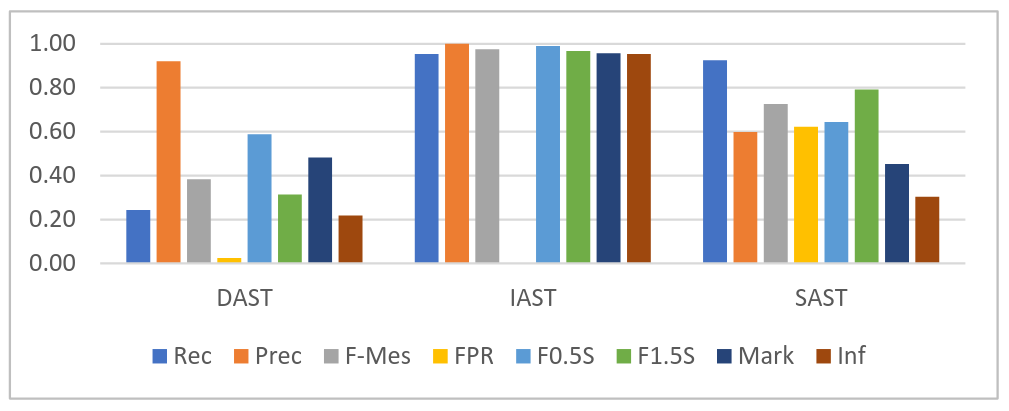
\includegraphics[width=0.9\linewidth]{images/AST_Comparison.png}
	\caption{Scrum4Safety Prozess}
	\label{fig:astCompare}
\end{figure}


\begin{figure}[H]
	\centering
	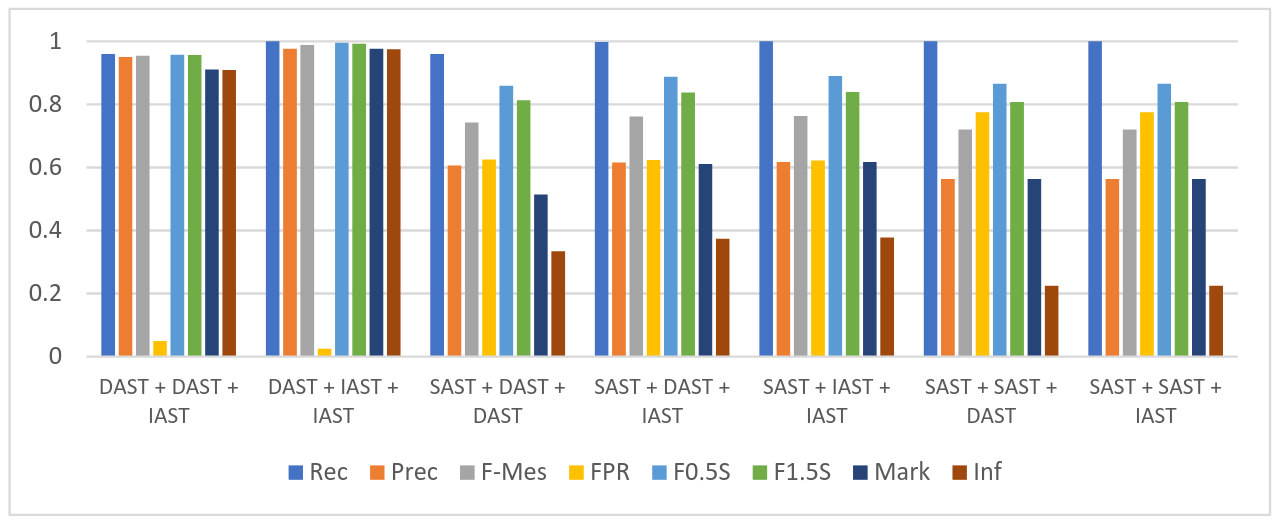
\includegraphics[width=0.9\linewidth]{images/AST_Comparison_Combination.png}
	\caption{Scrum4Safety Prozess}
	\label{fig:astCompareCompination}
\end{figure}

\subsection{Scrum4Safety}

Scrum4Safety verfolgt das Ziel, die Innovationsfähigkeit und Effizenz von agilen Methoden mit den strengen Anforderungen an Sicherheit und Konformität zu kombinieren.
Dafür führt es spezifische Rollen, Prinzipien und Workflows ein, um die Qualität und Sicherheit der zu entwickelnden Software sicherzustellen. Das Framework
erweitert die klassischen Scrum-Rollen um zusätzliche Rollen, die in sicherheitskritischen Projekten notwendig sind. Dabei handelt es sich um Verifier, Validator und Assessor.
Diese Rollen sind für den Quality-Assurance-Prozess verantwortlich und überprüfen die Einhaltung der Sicherheitsanforderungen. 

Neben den zusätzlichen Rollen führt Scrum4Safety auch neue Konzepte ein, die die Sicherheit der Softwareentwicklung gewährleisten sollen. Dazu gehört das Sprint-Hardening,
welches sicherstellen soll, dass am Ende jeder Iteration eine validierte Softwareversion bereitsgestellt werden kann. Dafür wird in jeder Iteration darauf geachtet, 
dass Benutzerdokumentationen und Konformitätsnachweise erstellt werden, die dann für die externe Softwarebewertung verwendet werden können. 
Ein weiteres Konzept ist die Continuous Compliance. Das beinhaltet, dass kontinuierlich Verfifizierungs- und Validierungsaktivitäten durchgeführt werden, sodass die Software
jederzeit konform ist. Dadurch sollen kritische Fehler frühzeitig erkannt werden, um sie schnellstmöglich beheben zu können. Das dritte Konzept ist die Living Traceability.
Durch die Einführung einer klaren Rückverfolgbarkeit in jedem Prozess bei der Umsetzung von Benutzeranforderungen soll die Zertifizierung 
der Software durch externe Prüftstellen erleichert werden. \cite{andriadi_impact_2023}

Der zentrale Prozess in Scrum4Safety ist der sogennante Safe-Sprint. Dabei handelt es sich wie beim klassischen Scrum-Prinzip um eine zeitlich begrenzte Iteration, in 
der ein neues Software-Inkrement entwickelt wird. Im Gegensatz zum klassischen Scrum soll das entwickelte Inkrement aber durch die eingeführten Konzepte sicherheitstechnisch
validiert sein. Dafür setzt Scrum4Safety mit dem Safe-Sprint schon in der Planning-Phase an und integriert Safety-Stories neben den klassischen User-Stories in den Backlog.
Dadurch soll gewährleistet sein, dass Sicherheit bereits in der Anforderungsphase berücksichtigt wird. Auch eine frühe Einbindung von Sicherheitsüberprüfungen und Testphasen im Ablauf 
des Safe-Sprints soll sicherstellen, dass Sicherheitsmaßnahmen frühzeitig in den Entwicklungsprozess integriert werden. 

\begin{figure}
  \centering
  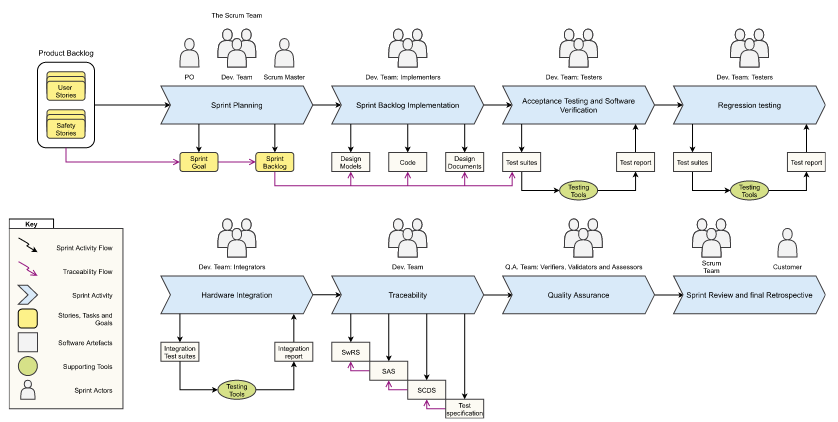
\includegraphics[width=0.9\linewidth]{images/S4S-Safe-Sprint.png}
  \caption{Scrum4Safety Prozess}
  \label{fig:scrum4safety}
\end{figure}



\section{Diskussion}

(Einordnung, Interpretation und Bewertung der Erkenntnisse -- (nachvollziehbare, begründbare) Meinungen sind erlaubt) 



\section{Zusammenfassung und Ausblick}

(Überblick über die gesamte Arbeit, Rückführung auf Aussagen aus Kapitel 1 durchführen, offene Punkte als neue Forschungsfragen definieren)



%% The next two lines define the bibliography style to be used, and
%% the bibliography file.
\bibliographystyle{ACM-Reference-Format}
\bibliography{08-Security-Software}

%%
%% If your work has an appendix, this is the place to put it.
\appendix

\section{Anhang 1}



\end{document}
\endinput
%%
%% End of file `sample-acmtog.tex'.
